\section{Einleitung}
Dieses Handbuch zeigt Schritt für Schritt auf, wie ownCloud auf einem Computer installiert und eingesetzt werden kann.
Es wird dabei nur für die Verwendung in einem Heimnetzwerk eingerichtet. Das bedeutet, dass man sich mit der Cloud verbinden kann, wenn man sich in seinem lokalen Netzwerk befindet. Um von ausserhalb - beispielsweise von einem Smartphone - darauf zuzugreifen, benötigt es weitere Schritte, die in diesem Tutorial nicht abgedeckt werden. Es wird aber an den entsprechenden Stellen auf hilfreiche Ressourcen verwiesen.

\section{Raspberry Pi}
Ein Raspberry Pi ist ein Einplatinencomputer in der Grösse einer Kreditkarte.
Er wurde 2009 von der Raspberry Pi Foundation entwickelt, um Schulen einen kostengünstigen Computer zur Verfügung zu stellen.
Dabei ging es vor allem um das Erlernen von Computerwissenschaften, wie Programmierung von Software oder Ansteuerung einfacher Hardware, wie LEDs, Displays und einfachen Motoren.
\footnote{\url{http://www.raspberrypi.org/faqs\#introWhatIs}}
\footnote{\url{http://www.raspberrypi.org/about}}
Der Raspberry Pi ist sehr vielseitig einsetzbar und nicht zuletzt deswegen hat sich eine grosse und begeisterte Community gebildet. Als Betriebssystem kommt auf Grund der leistungsfähig begrenzten Hardware meistens eine Linux-basierte Distribution zum Einsatz. Linux arbeitet sehr ressourcenschonend und die Distributionen sind zudem oft speziell auf den Rechner und das jeweilige Einsatzgebiet angepasst.
Der Raspberry Pi ist ein Spielzeug für technikbegeisterte Menschen - jung und alt gleichermassen. Die Community ist ein essentieller Bestandteil des Projektes, denn sie erfinden ständig neue Einsatzmöglichkeiten, kreieren interessante Produkte und Projekte und stellen Anleitungen ins Netz. Um dann selbst loszulegen, braucht man oft nicht mehr als den Raspberry Pi selbst, Monitor, Tastatur und Maus und ein wenig Know-How.

\subsection{Hardware}
Es ist wichtig, für die Inbetriebnahme des Raspberry Pis ein wenig über die Hardware Bescheid zu wissen.
Es gibt zur Zeit zwei Modelle des Mini-Rechners: das ursprüngliche Model A und das erweiterte Model B. Model B ist performanter und verfügt über mehr Anschlüsse. Aus diesem Grund ist es Model A in den meisten Fällen vorzuziehen.

Raspberry Pi, Model B verfügt über folgende Anschlüsse:

\begin{itemize}
  \item Kartenleser für SD/MMC/SDIO (Hauptspeicher, Betriebssystem)
  \item 2x USB 2.0
  \item FBAS (Videoausgabe)
  \item HDMI (Video \& Audio)
  \item Klinkenstecker, 3.5mm (Audio)
  \item 10/100-MBit Ethernet Controller (RJ45, Netzwerk)
  \item 17 GPIO Pins (Externe Hardware)
  \item 5V Micro-USB (Stromanschluss)
\footnote{\url{http://de.wikipedia.org/wiki/Raspberry_Pi\#Spezifikationen}}
\end{itemize}

\begin{figure}[h]
  \centering
  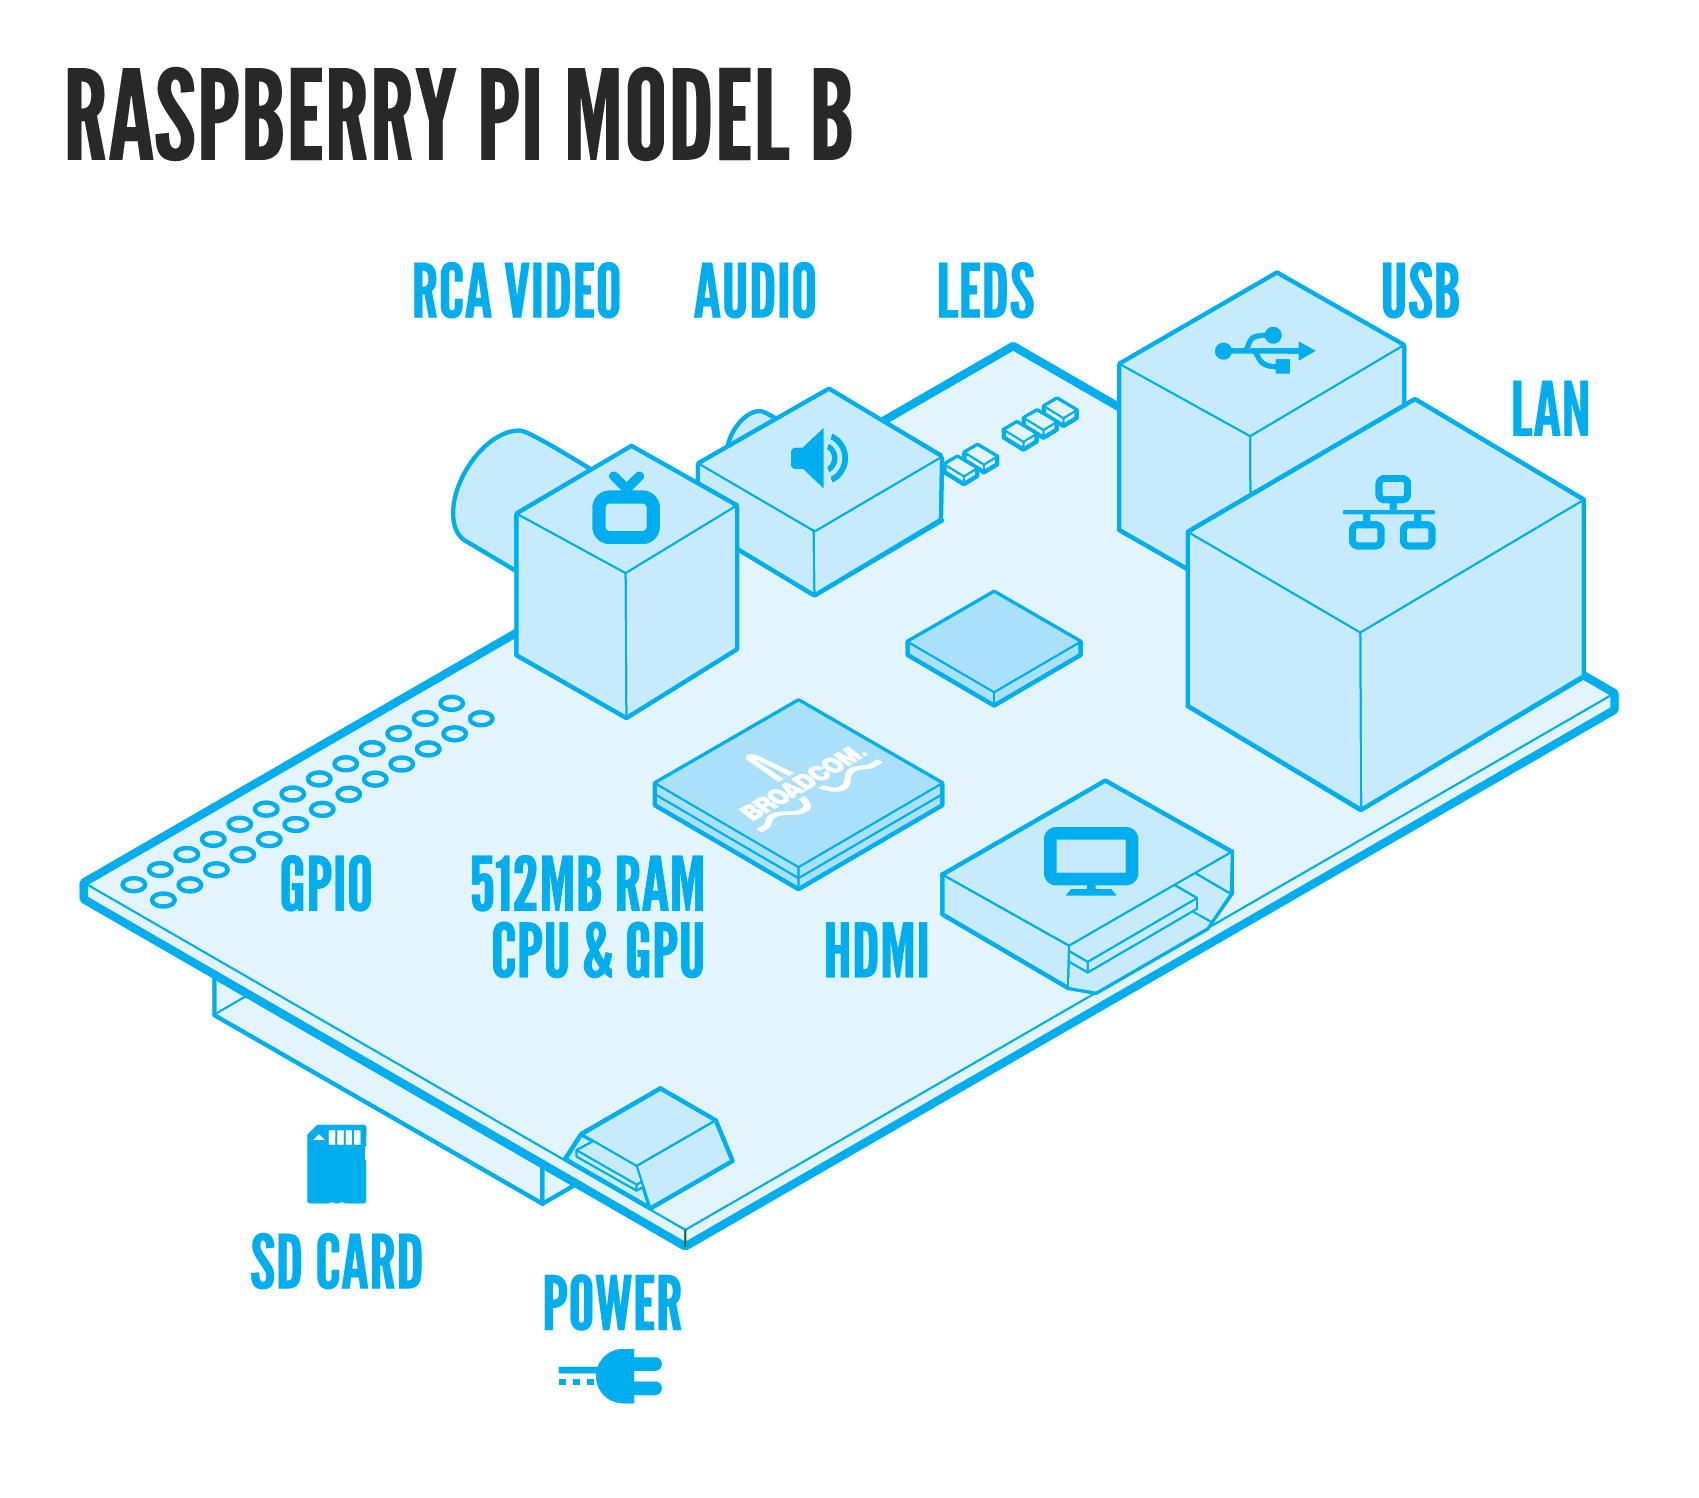
\includegraphics[scale=0.50]{../images/RaspiModelB}
  \caption{Raspberry Pi, Model B}
\end{figure}

\subsection{Betriebssystem}
Wie bereits erwähnt, wird in diesem Versuch eine Linux-basierte Distribution eingesetzt, die speziell auf den Raspberry Pi zugeschneidert wurde. Raspbian basiert auf der Linux-Distribution Debian und ist neben den Grundfunktionalitäten mit vielen weiteren Programmen ausgestattet, die ``out of the box'' genutzt werden können.
\footnote{\url{http://www.raspbian.org/}}
Wie die meisten anderen Linux-basierten Distributionen, kann Raspbian gratis aus dem Internet heruntergeladen und eingesetzt werden. Natürlich ist es nicht das einzige Linux-Betriebssystem, welches auf dem Raspberry Pi eingesetzt werden kann. Eine Liste bekannter Distributionen kann unter \url{http://www.raspberrypi.org/downloads} gefunden werden.

